%%%%%%%%%%%%%%%%%%%%%%%%%%%%%%%%%%%%%%%%%%%%%%%%%%%%%%%%%%%%%%%%%%%%%%%%%%%%%%%%%%%%%%%%%%%%%%%%%%%%%%%%%%%%%%%
\chapter{SLM energy preservation}
%%%%%%%%%%%%%%%%%%%%%%%%%%%%%%%%%%%%%%%%%%%%%%%%%%%%%%%%%%%%%%%%%%%%%%%%%%%%%%%%%%%%%%%%%%%%%%%%%%%%%%%%%%%%%%%
It can be proved that a restart of SLM does not alter the energy. This chapter is devoted to showing that this is true.

The residual energy of the symplectic Lanzcos method is
\begin{equation}
\frac{1}{2} e_r^{\top} J A e_r + e_r^\top J r_{n+1} e_{2n}^\top z
\end{equation}
with $ e_r = y-y_n $ (analytical solution minus approximated solution) and $r_{n+1}$ is the residual vector given by the symplectic Lanzcos method. 

\begin{figure}[H]
        \centering
        \begin{subfigure}[b]{0.45\textwidth}
                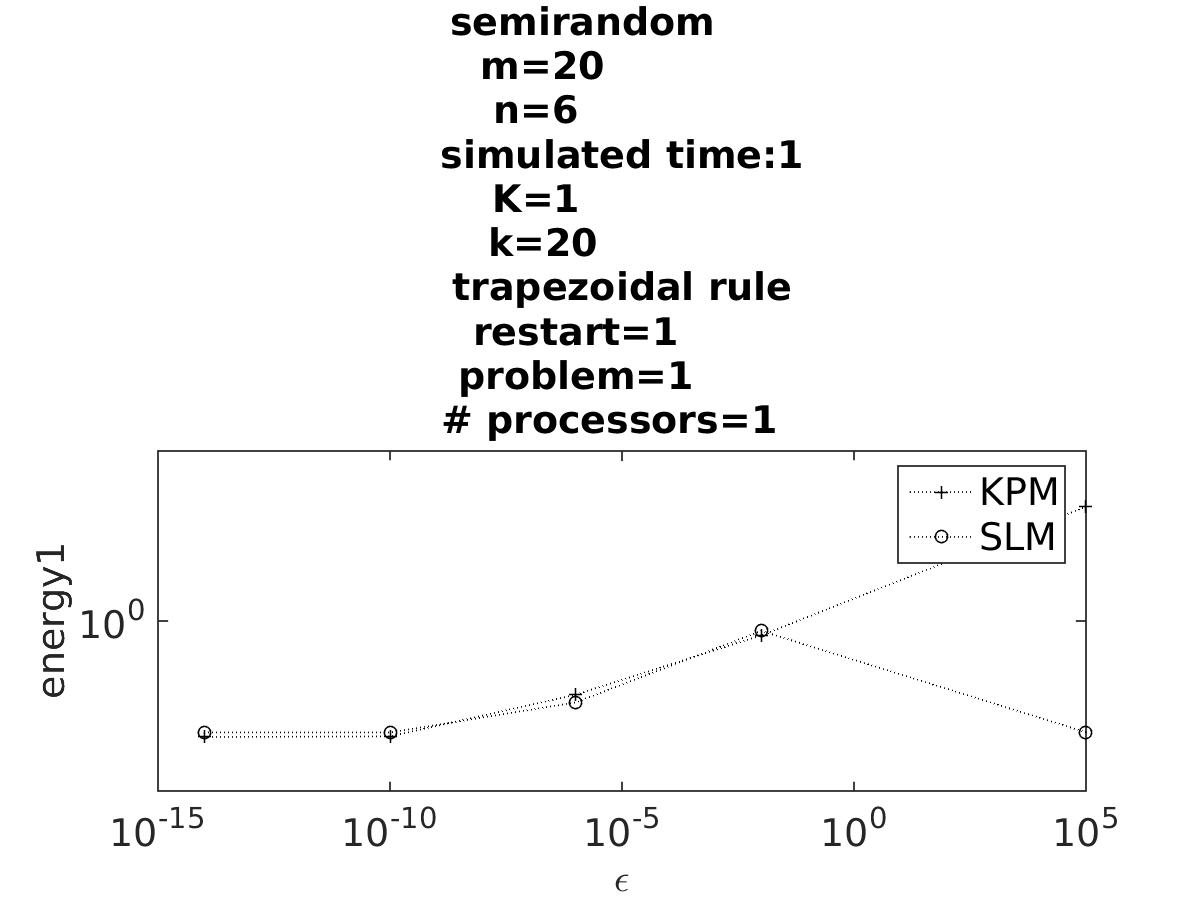
\includegraphics[width=\textwidth]{../MATLAB/fig/compareEnergy.jpg}
                \caption{ Tekst her! }
                \label{fig:intconvtrap}
        \end{subfigure}%
        ~
        \begin{subfigure}[b]{0.45\textwidth}
                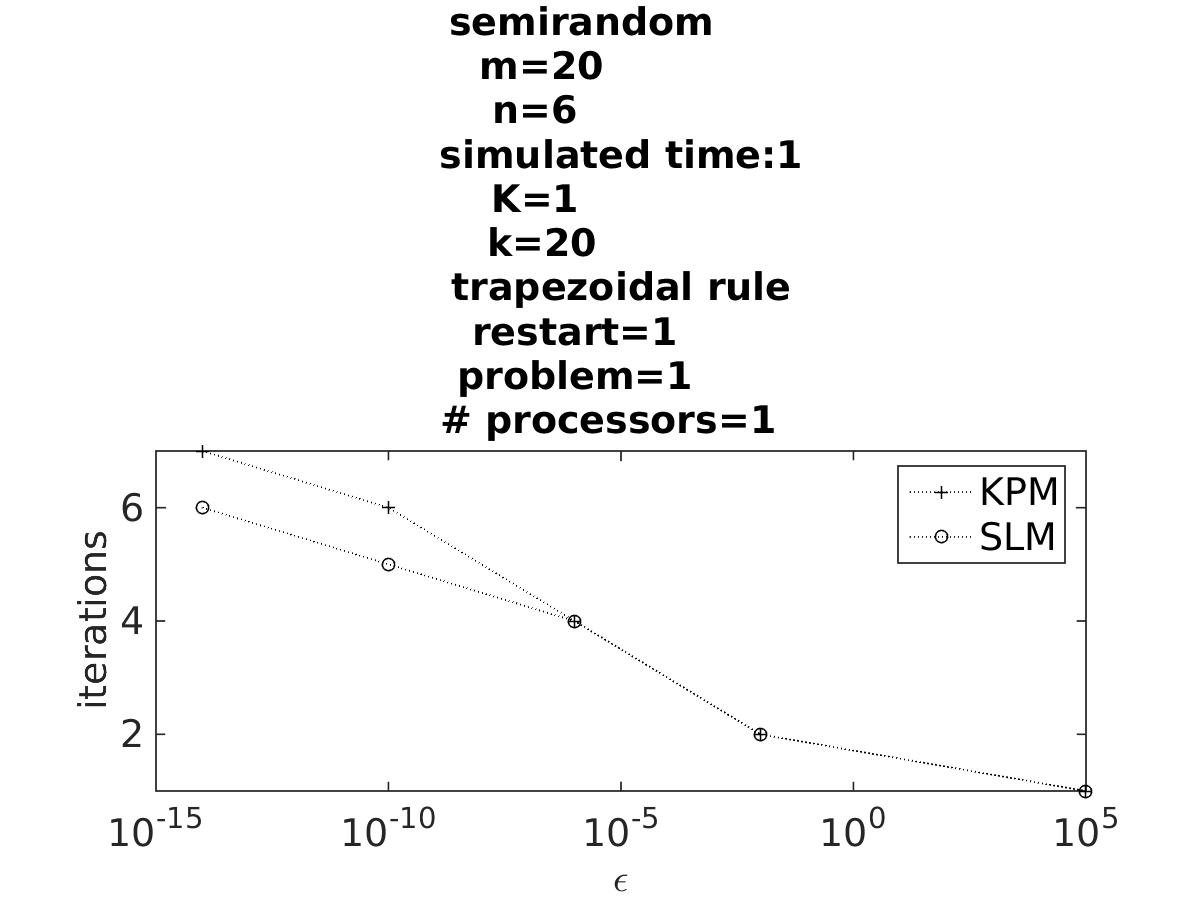
\includegraphics[width=\textwidth]{../MATLAB/fig/compareIter.jpg}
                \caption{ Tekst her! }
                \label{fig:intconveul}
        \end{subfigure}
        \caption{Tekst her! }
        \label{fig:intconv}
\end{figure}

The figures above implies that restarting the symplectic Lanzcos method does indeed not change the energy. But for Arnoldi's method it changes quite a bit. 

The figures below shows the difference between the symplectic Lanczos method with and without restart. 
\begin{figure}[H]
        \centering
        \begin{subfigure}[b]{0.45\textwidth}
                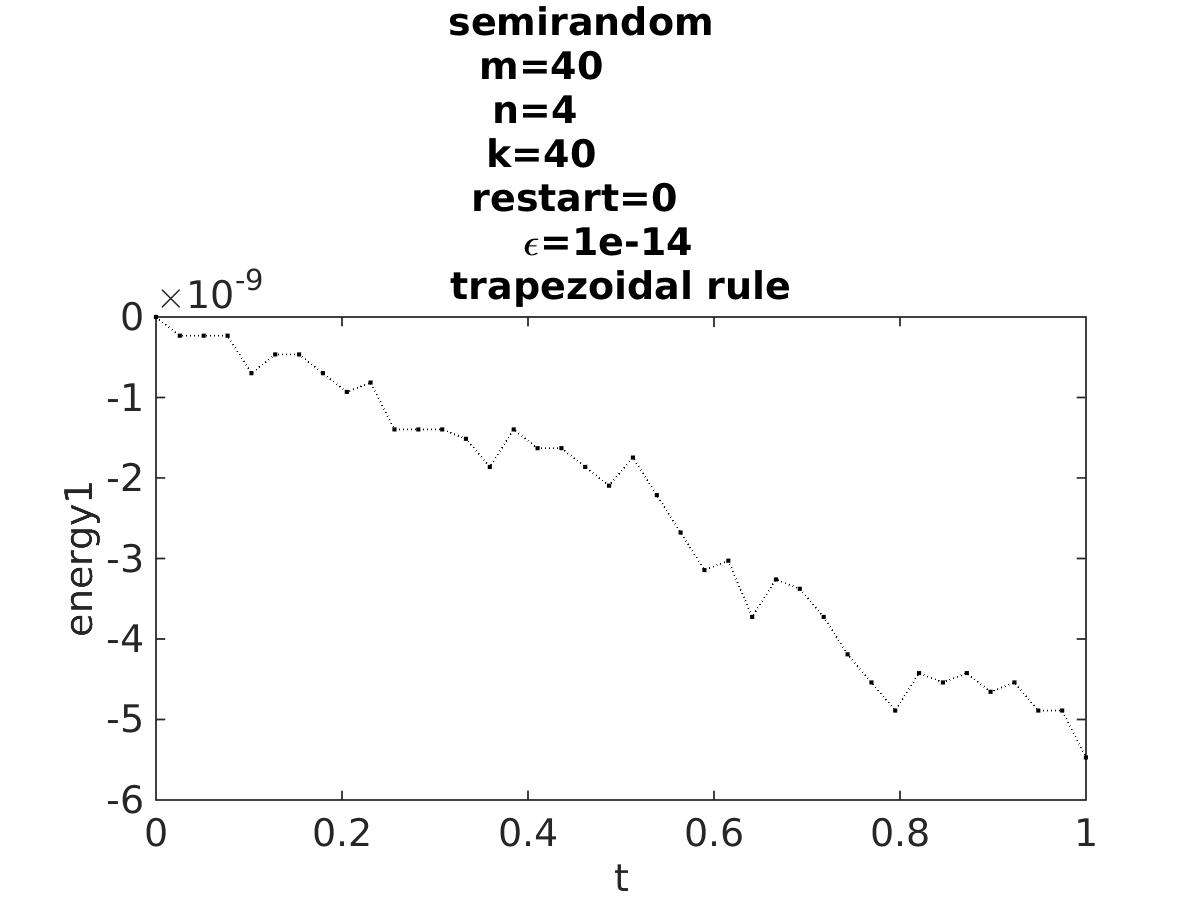
\includegraphics[width=\textwidth]{../MATLAB/fig/energytestrestart0.jpg}
                \caption{ Without restart. Tekst her! }
                \label{fig:intconvtrap}
        \end{subfigure}%
        ~
        \begin{subfigure}[b]{0.45\textwidth}
                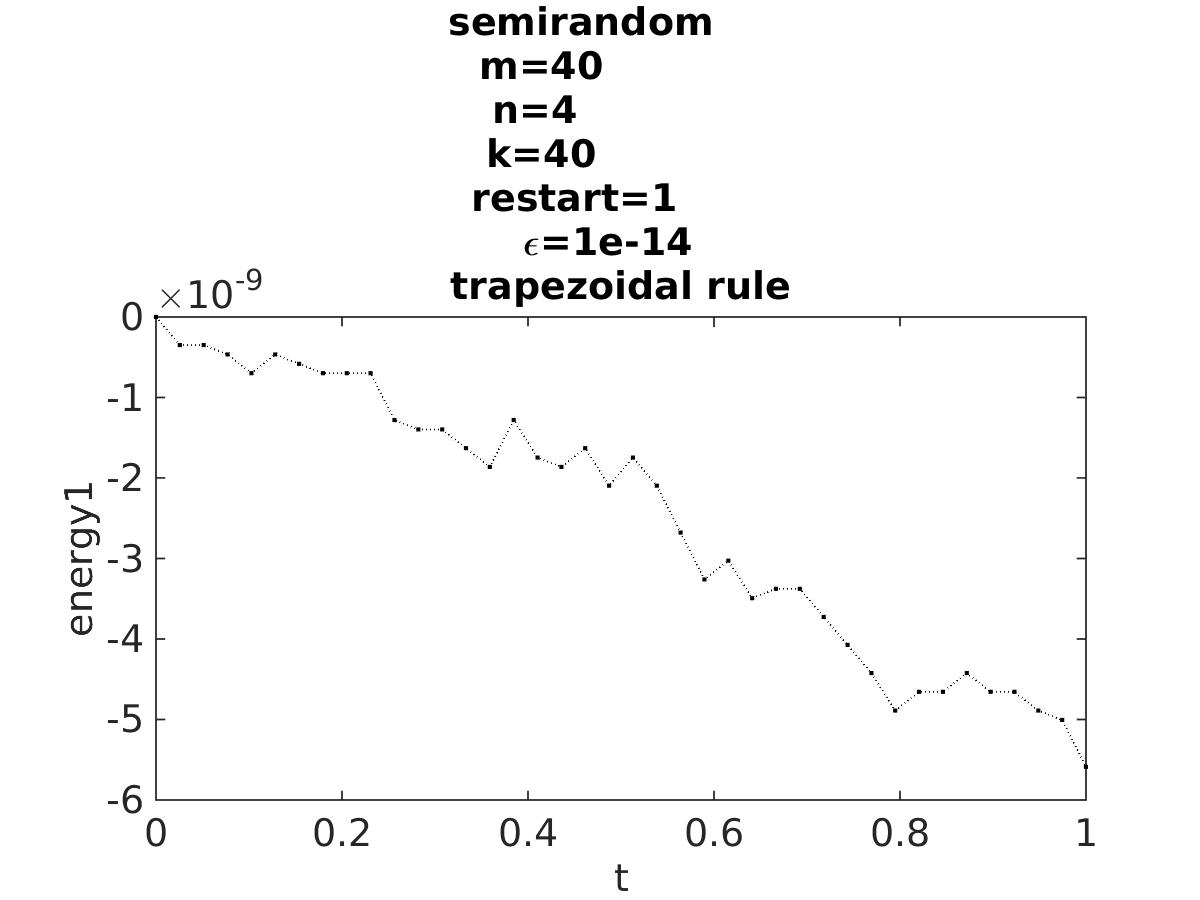
\includegraphics[width=\textwidth]{../MATLAB/fig/energytestrestart1.jpg}
                \caption{ With restart.  Tekst her! iter = 47 }
                \label{fig:intconveul}
        \end{subfigure}
        \caption{ The figures shows the change in energy over time. Mer tekst  }
        \label{fig:intconv}
\end{figure}
The figure above shows very little difference in energy with SLM, even with several restarts. \\


!!!!!!!!!!!!!!!!!!!!!!!!!!!!!!!Bilde av hvordan dette ser ut for arnoldi?!!!!!!!!!!!!!!!!!!!!!!!!!!\\

!!!!!!!!!!!!!!!!!!ARG, hva må jeg ha med for at dette skal bli mer overbevisende?!!!!!!!!!!!!!!!!!!!!!

